% \Huge

\todo[inline]{The section names here are just temporary.}

\section{Method}

\todo[inline]{Present how we did the perfect reconstruction}

The first step in understanding the evolution of the universe is to look at the theoretical limits we encounter when trying to reconstruct it. As a field is defined at every point in space, any attempt at representing it with data is inherently imperfect. We would have to measure the density field at every point in the Universe in order to obtain all the information it contains. This fact already implies that no data driven reconstruction will ever succeed at perfectly recovering the primordial density field (unless we manage to make an infinity of measurements). 

To show this unavoidable loss of information we performed a `perfect' reconstruction. We have access to multiple snapshots at various redshifts in our simulations, including the initial positions of all particles (at $z = 99$). Therefore, we used this information to reconstruct the density field. We first calculated the density field at various redshifts in the interval $z = 0 - 9$. The field was calculated at the particle positions instead of being calculated on a regular grid. This is because we want the particles to carry the density field when we move them. After that, all the particles were moved to their initial positions at $z = 99$.

The density field is carried by the particles to $z = 99$. As the particle distribution was almost perfectly uniform at the beginning, the density field will also be very uniform. However, this procedure also creates an interesting side effect. At late time, most particles tend to be clumped together. Therefore, when measuring the density field at the particle positions, we will mostly get very high values. These values don't change when moving the particles, so the final field will also have very high values, but this time distributed on an almost uniform grid. This results in an apparent increase in the total mass of the simulation. As this increase is just a result of the way we represent the density field, it needs to be accounted for when analysing the results. The total mass of the simulation should be conserved. 

\section{Results}

\todo[inline]{Show some density slices of the results, and talk about the effects that pop up (e.g. the increase in total mass). Show Power Spectra}

\begin{figure}
    \centering
    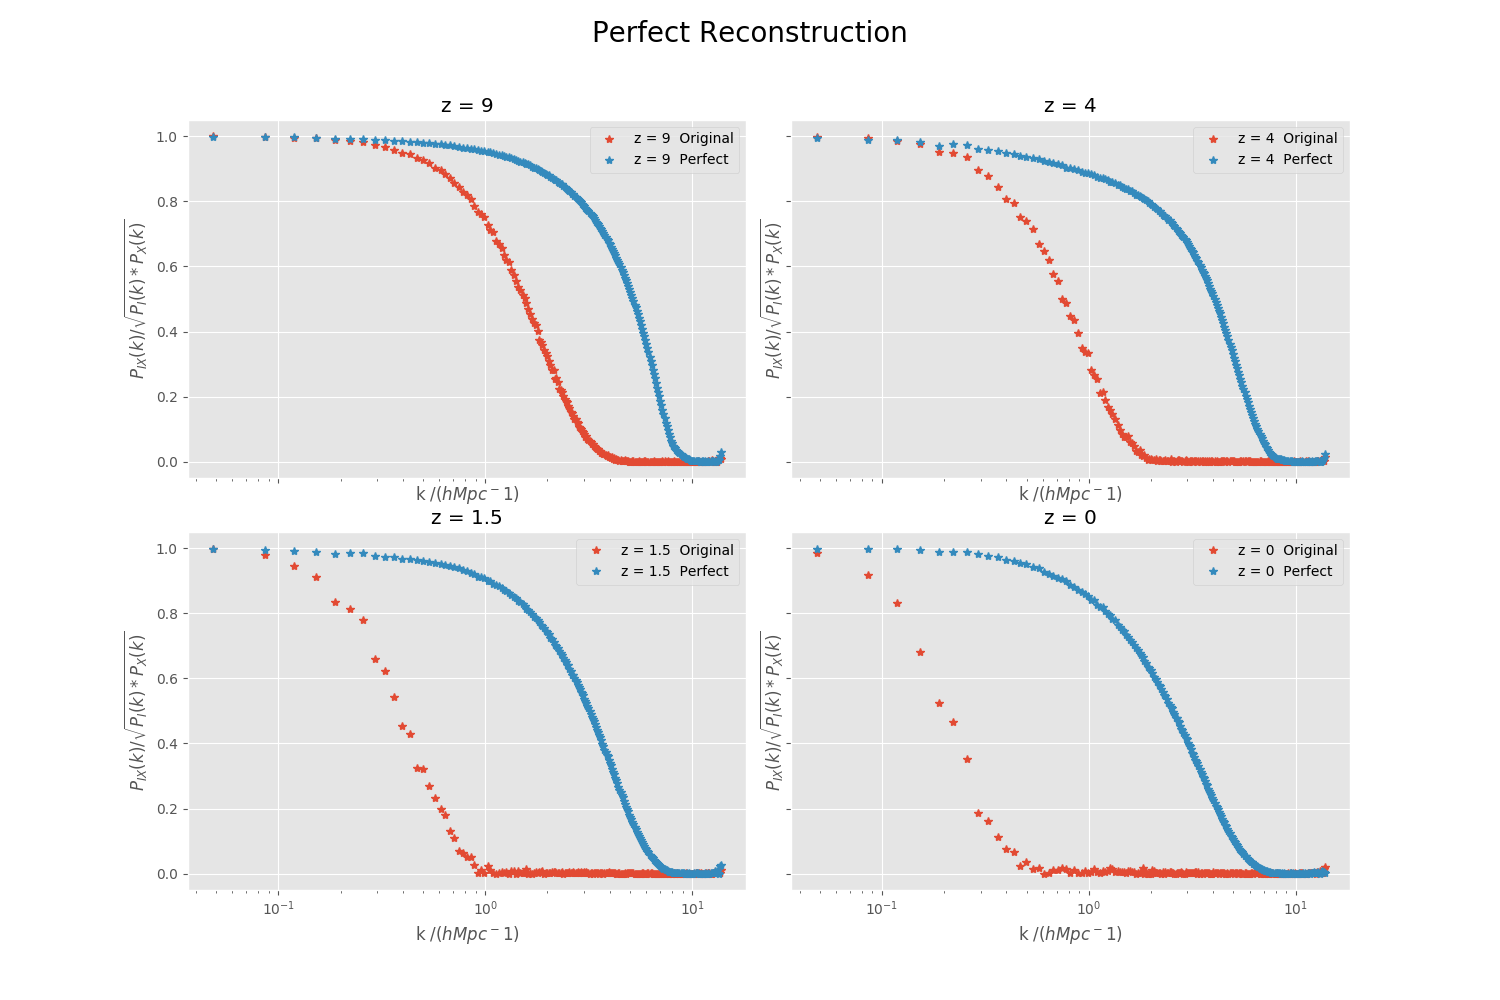
\includegraphics[width=1\columnwidth]{images/crossSpectra/Spec_1_perf.png}%
    
    \caption{
    Comparison between the original and perfect reconstruction cross-Spectra at different redshifts. 
    }
    
    \label{fig:4}
\end{figure}

\section{Analysis}

\todo[inline]{Present Cross-Spectra and talk about how well this worked and the weird effect around z=4.}

\todo[inline]{Sim A: $(200 Mpc)^3$, $512^3$ Particles

Sim B: $(200 Mpc)^3$, $256^3$ Particles

Sim C: $(100 Mpc)^3$, $256^3$ Particles}

\begin{figure}
    \centering
    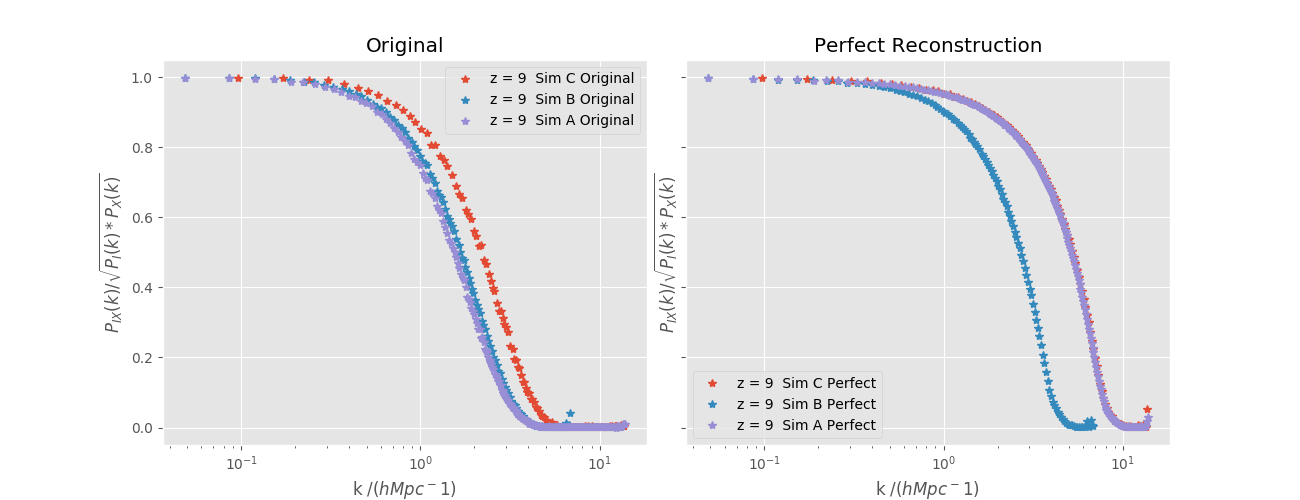
\includegraphics[width=1\columnwidth]{images/crossSpectra/Spec_2_perf.png}%
    
    \caption{
    Comparison between different simulations of the original and the reconstructed correlation. 
    }
    
    \label{fig:5}
\end{figure}

\begin{figure}
    \centering
    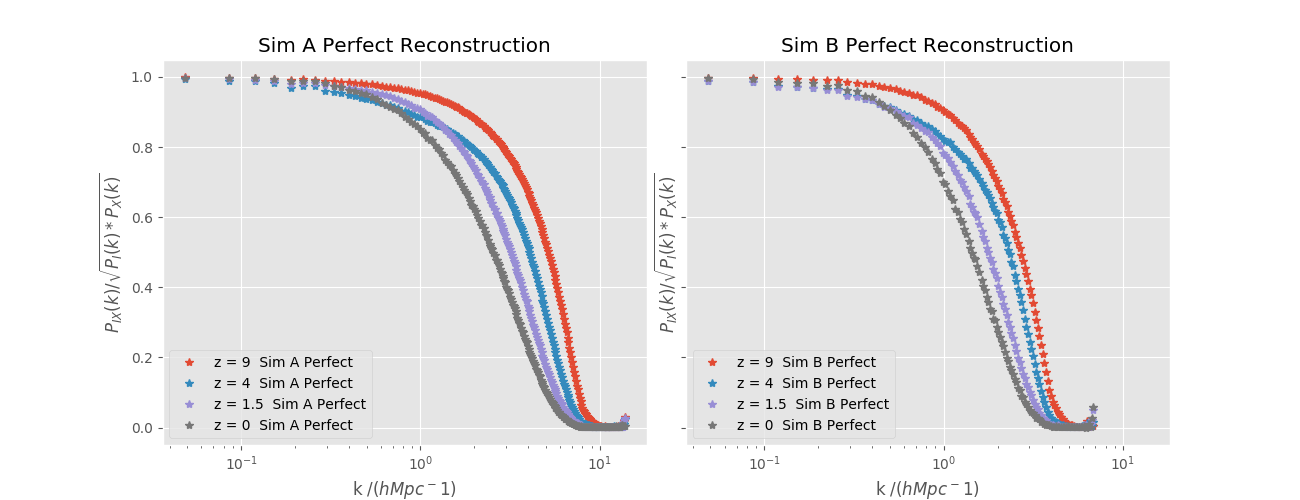
\includegraphics[width=1\columnwidth]{images/crossSpectra/Spec_3_perf.png}%
    
    \caption{
    Perfect Reconstruction from different redshifts in Sim A and Sim B
    }
    
    \label{fig:6}
\end{figure}